\documentclass{article}

\usepackage{float}
\usepackage{amsmath}
\usepackage{amsfonts}
\usepackage{amssymb}
\usepackage{graphicx}
\usepackage[margin=1in]{geometry}

\usepackage[backend=biber, style=alphabetic, sorting=ynt]{biblatex}

\addbibresource{references}
  
\title{Week 3 - Homework}
\author{Artur Topal, S5942128}
\date{\today}

\begin{document}

\maketitle

\begin{center}
  \textbf{TA}: Hanna, grp\_356739\_6
\end{center}

\pagebreak

\section{ Problem H1 } 
Given:
\begin{equation} \label{eq:surface_equation}
4x^2 + y^2 + 4z^2 = 16, z \ge 0
\end{equation}

Due to gravity, a raindrop moves along the path on the surface Eq.~\eqref{eq:surface_equation} so that its vertical component ($z$) decreases the quickest. From Eq.~\eqref{eq:surface_equation}, derive $z$:
\begin{equation*}
  z \ge 0 \Rightarrow z(x, y) = \frac{1}{2}\sqrt{16 - 4x^2 - y^2}
\end{equation*}

Suppose a raindrop moves along some curve $\vec{r}(t) = (x(t), y(t))$ that lies on the surface (Eq.~\eqref{eq:surface_equation}). Then, there is a number of ways to calculate this curve. For instance, Newton's second law will produce $\vec{r}(t)$ with time evolution, however it will require numerical methods. For the purposes of this paper, time information is sacrificed to facilitate analytical methods.

\begin{figure}[H]
  \centering
  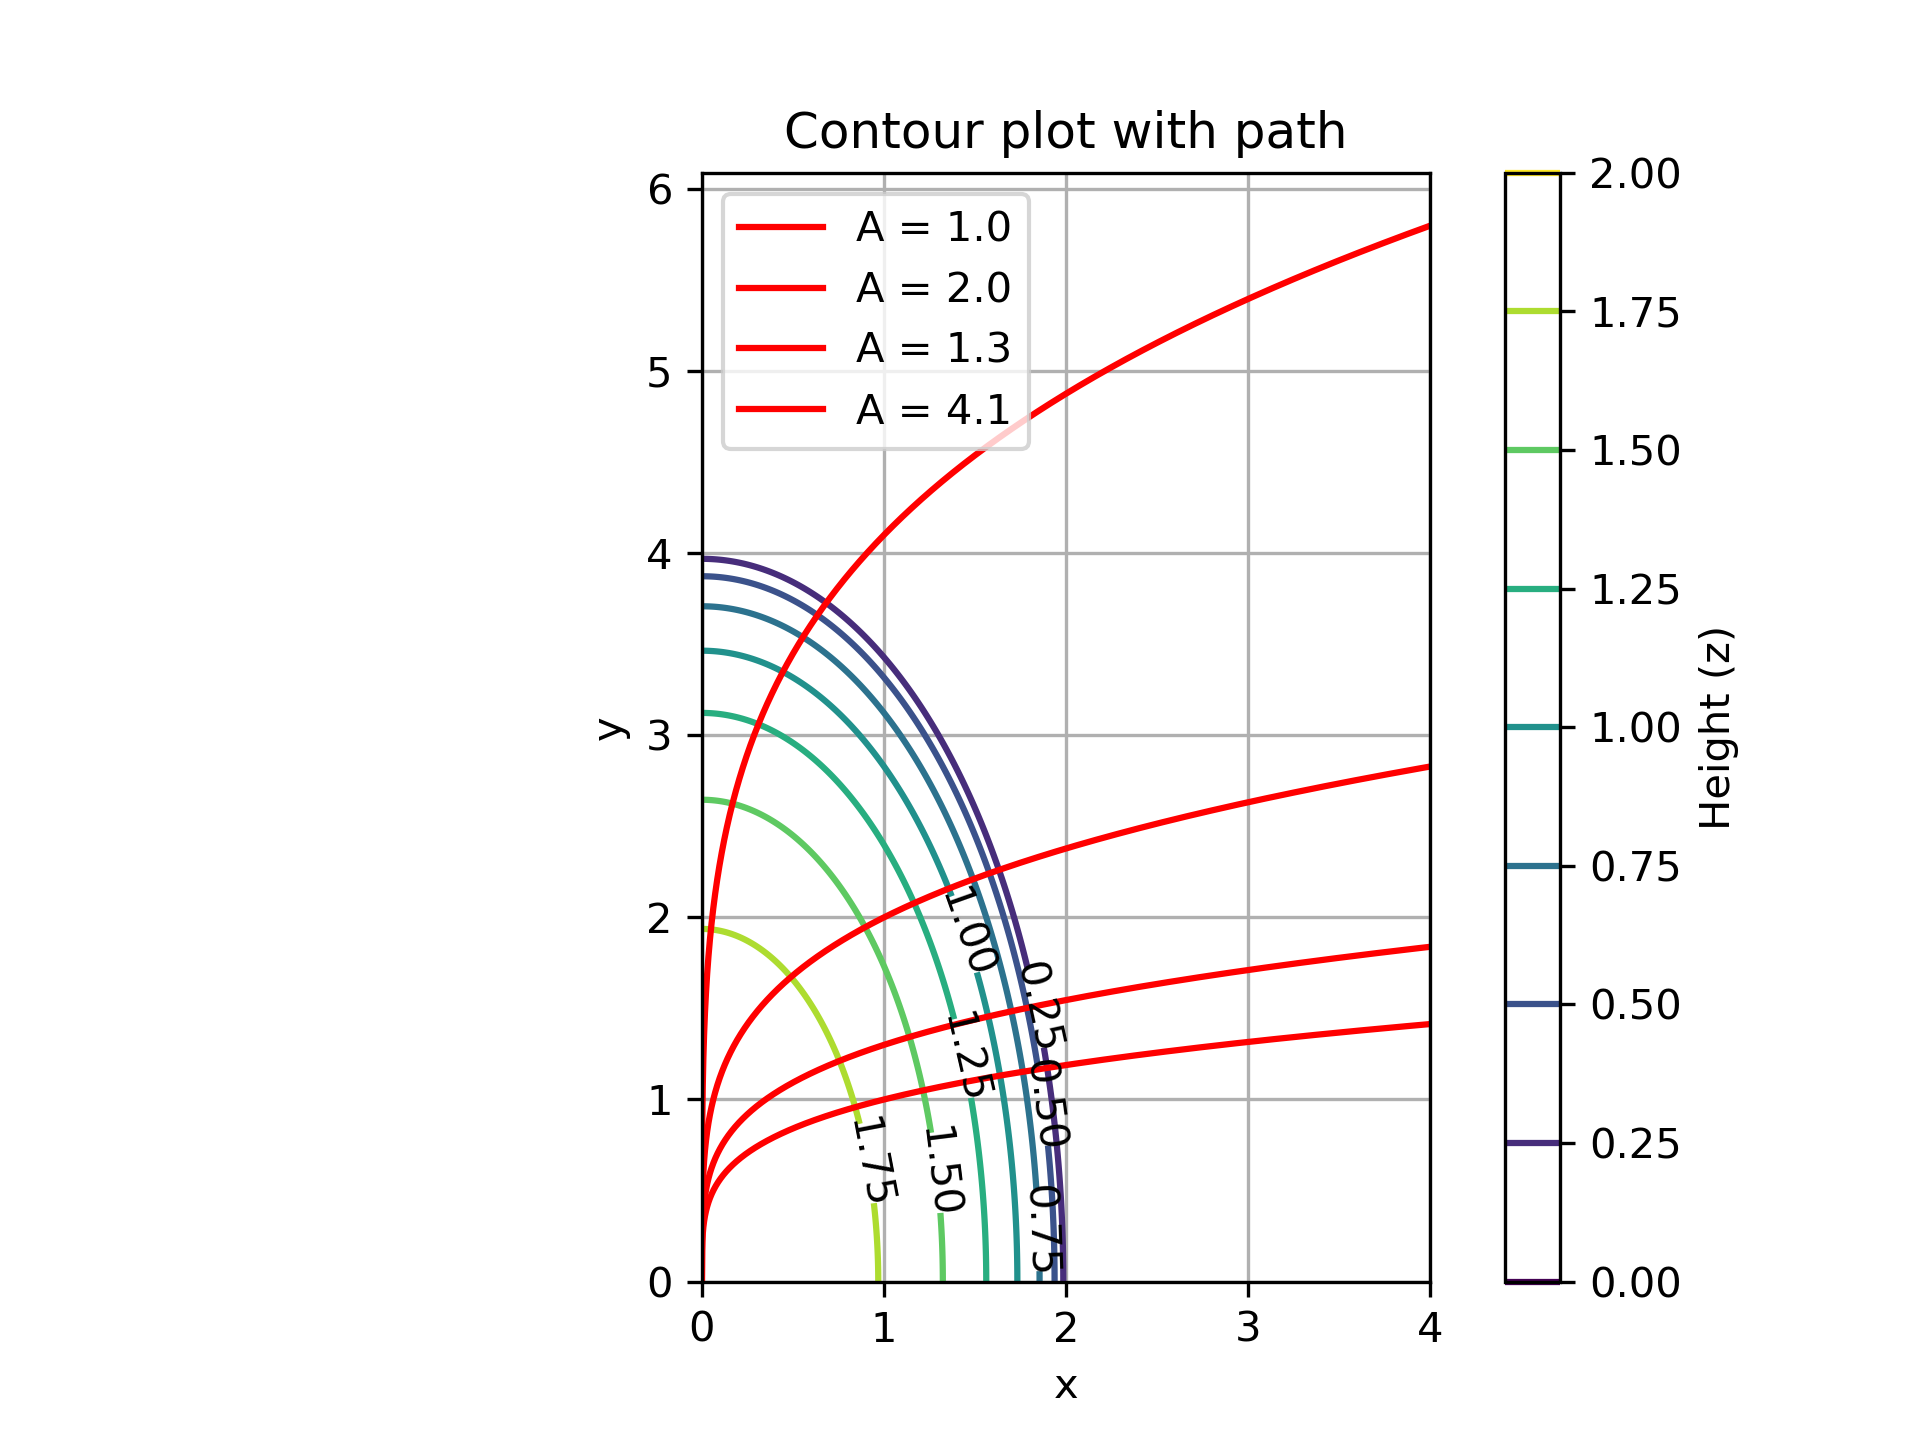
\includegraphics[width=0.7\textwidth]{calculus/W3/img/raindrop.png}
  \caption{Level curves, and raindrop's steepest path with different values for A.}
  \label{fig:raindrop_path}
\end{figure}

Level curves of $z(x, y)$ and the desired path $\vec{r}(t)$ for different values of parameter $A$ (see Eq.~\eqref{eq:curve}) are depicted in Fig.\ref{fig:raindrop_path}\footnote{We will find $\vec{r}(t)$ in terms of $x$ and $y(x)$, and then associate $z$ values for each pair $(x, y(x))$.}. From the figure, it is clear that at each point of the path, its tangent is collinear with the gradient of $z(x, y)$. This is true because the negative gradient points in the direction of the steepest descent. This consideration results into:
\begin{equation*}
  \frac{d\vec{r}(t)}{dt} = - \mu \nabla{z} \Rightarrow (\dot{x}, \dot{y}) = \mu (z_x, z_y), \mu \in \Re^{+}
\end{equation*}

Divide the two components of the vectors and apply [the inverse of] the Chain Rule:
\begin{equation} \label{eq:main}
  \frac{dx}{dt} \frac{dt}{dy} = \frac{-\mu z_x}{-\mu z_y} \Rightarrow \frac{dy}{dx} = \frac{z_y}{z_x}
\end{equation}

Calculate partial derivatives of $z_x$ and $z_y$:
\begin{equation*}
  z_x = \frac{\partial}{\partial x}{ \frac{1}{2}\sqrt{16 - 4x^2 - y^2}} = \frac{-8x}{4 \sqrt{16-4x^2-y^2}} = -\frac{x}{z}
\end{equation*}
\begin{equation*}
  z_y = \frac{\partial}{\partial y}{ \frac{1}{2}\sqrt{16 - 4x^2 - y^2}} = \frac{-2y}{4 \sqrt{16-4x^2-y^2}} = -\frac{y}{4z}
\end{equation*}

Now, substitute those partial derivatives in Eq.~\eqref{eq:main}:

\begin{equation*}
  \frac{dy}{dx} = \frac{-y}{4z} \frac{z}{-x} = \frac{y}{4x}
\end{equation*}

Solve above derived equation by the separation of variables:

\begin{equation*}
  \int{\frac{dy}{y}} = \int{\frac{dx}{4x}} \Rightarrow ln(y) + C = \frac{ln(x)}{4} \Rightarrow y = e^{\frac{ln(x)}{4} - C} = e^{-C}e^{\frac{ln(x)}{4}}, x \ge 0
\end{equation*}

Thus,
\begin{equation} \label{eq:curve}
  y(x) = Ax^{1/4}
\end{equation}
where one can determine $A$  using the time information that was sacrificed to avoid numerical methods.

The curve in Eq~\eqref{eq:curve} can also be visualized on the surface of the roof of Eq~\eqref{eq:surface_equation}. To do so, vertical component $z$ must be found using curve's $(x, y) = (x, Ax^{1/4})$:
\begin{equation*}
  z(x) = z(x, y(x)) = \frac{\sqrt{16 - 4x^2 - y^2}}{2} = \frac{\sqrt{16 - 4(x)^2 - (Ax^{1/4})^2}}{2}
\end{equation*}
\begin{equation} \label{eq:raindrop_path_z}
  z(x) = \frac{\sqrt{16 - 4x^2 - A^2\sqrt{x}}}{2}
\end{equation}

\begin{figure}[H]
  \centering
  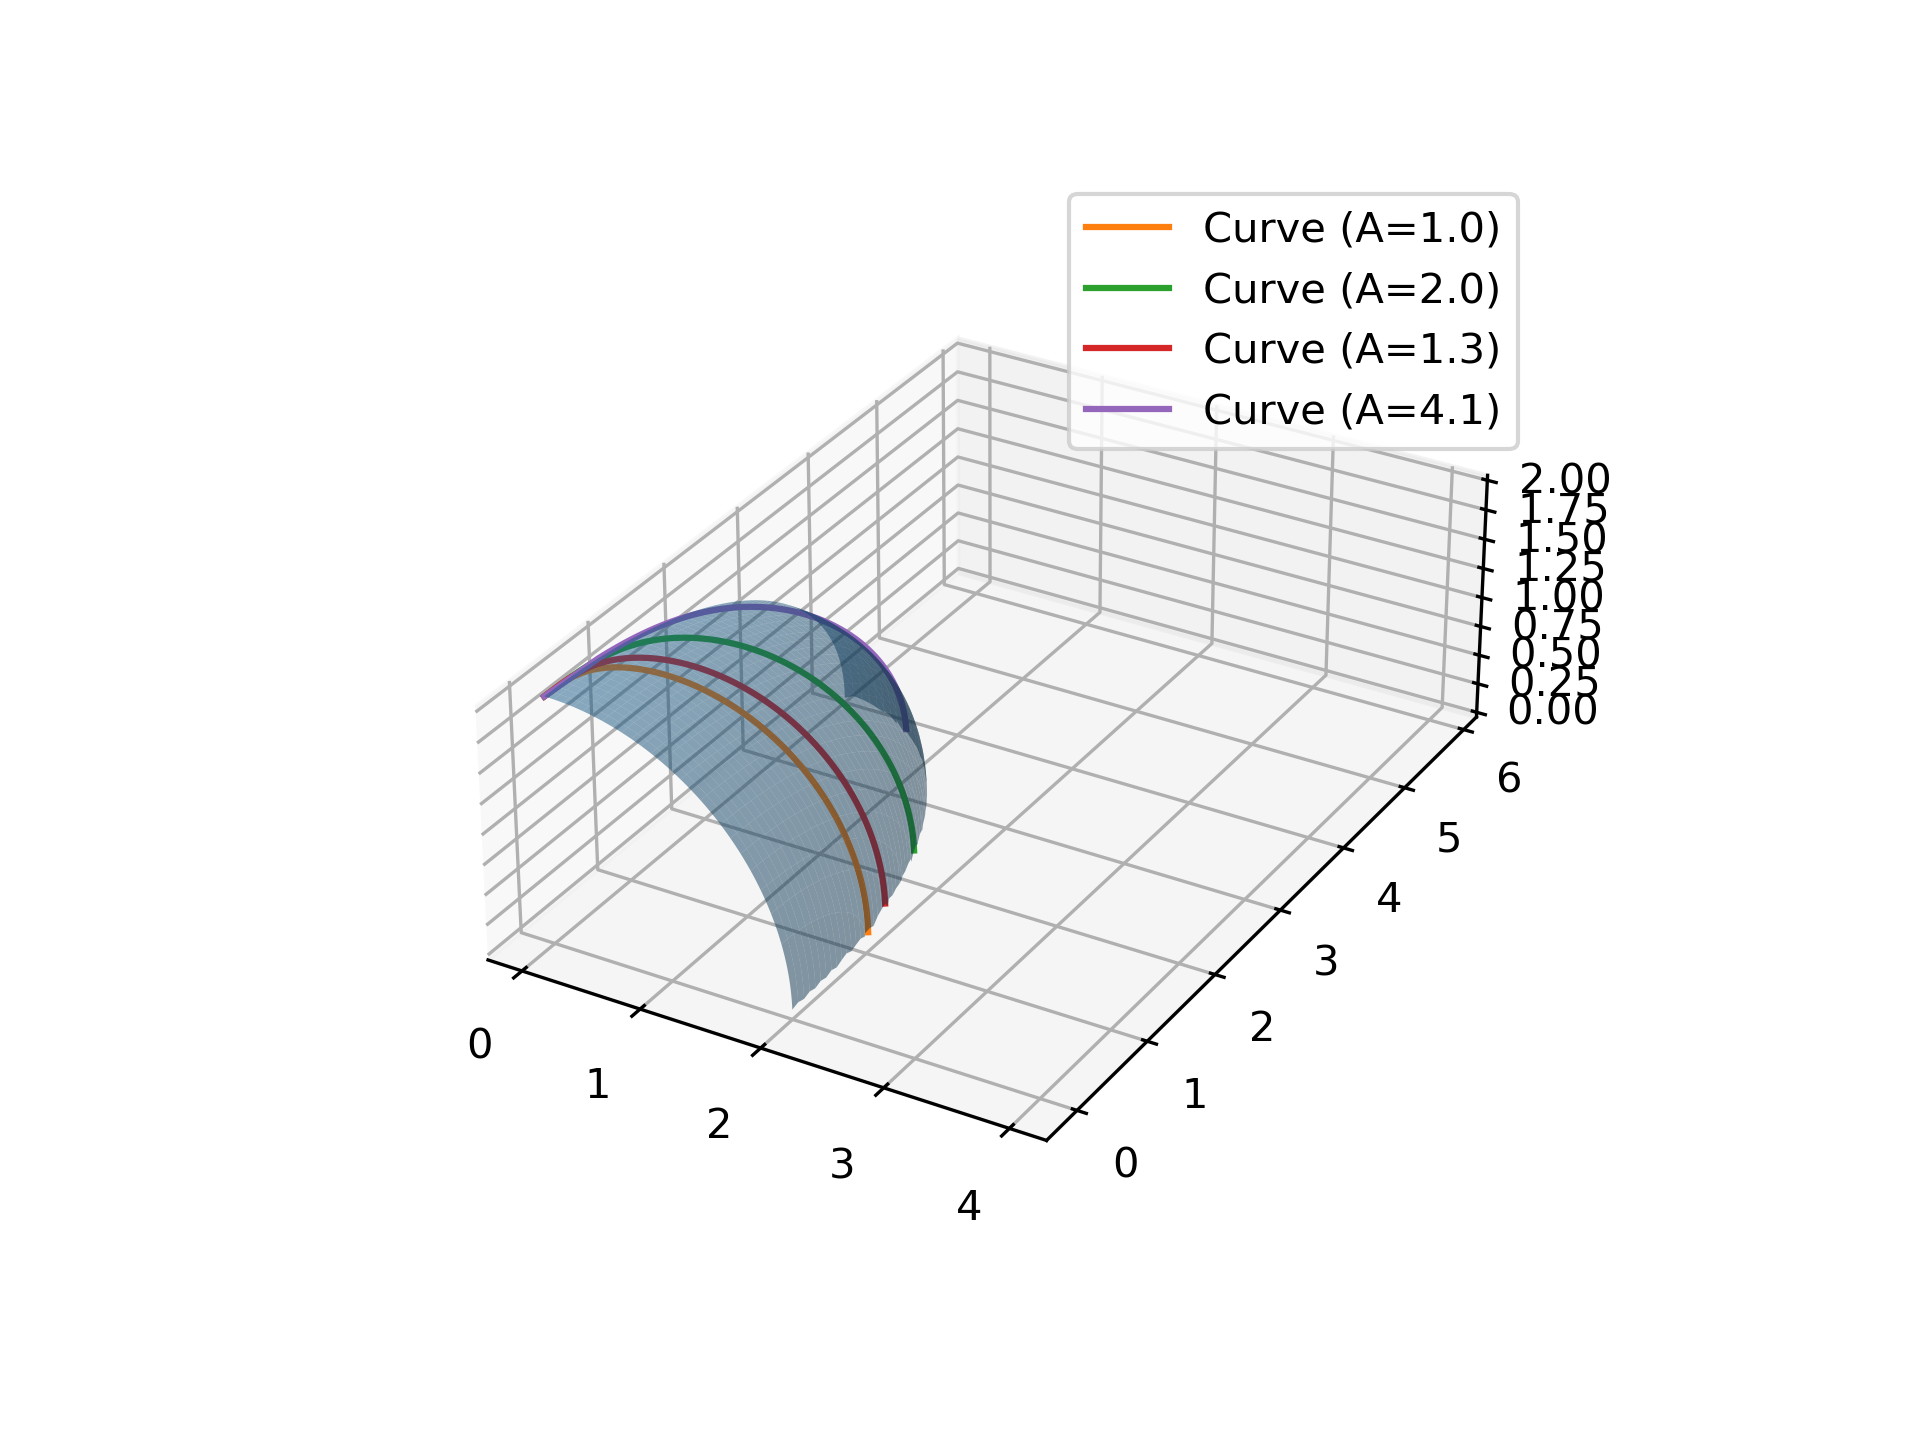
\includegraphics[width=0.5\textwidth]{calculus/W3/img/surface.png}
  \caption{Roof surface, and raindrop's steepest path for A=[1.0, 2.0, 1.3, 4.1]}
  \label{fig:surface}  
\end{figure}

Resultant raindrop's steepest path, described by Eq.~\eqref{eq:raindrop_path_z} and Eq.~\eqref{eq:curve} for different values of A, on the roof's surface described by Eq.~\eqref{eq:surface_equation} are depicted in Fig.\ref{fig:surface}\footnote{For code, refer to [2]}.

\hfill \break
\textbf{Answer}
\begin{equation*}
  y(x) = Ax^{1/4}, z(x) = \frac{\sqrt{16 - 4x^2 - A^2\sqrt{x}}}{2}
\end{equation*}

\section{ Problem H2 }

Given:
\begin{equation} \label{eq:stirling_of_W}
  S = kln(W)
\end{equation}

\begin{equation} \label{eq:energy_conservation}
  E = \sum_{i=1}^{3}{n_iE_i} = g(...n_i) 
\end{equation}

\begin{equation} \label{eq:number_conservation}
  N = \sum_{i=1}^{3}{n_i} = h(...n_i)
\end{equation}

\begin{equation} \label{eq:W_definition}
  W(n_1, n_2, n_3) = \frac{(n_1 + n_2 + n_3)!}{n_1!n_2!n_3!}
\end{equation}

First, substitute Eq.~\eqref{eq:W_definition} into Eq.~\eqref{eq:stirling_of_W} to find $S(W)$ in terms of $n_1, n_2, n_3$. Also, substitute Eq.~\eqref{eq:number_conservation}:
\[
  S(n_1, n_2, n_3) = kln \frac{(n_1 + n_2 + n_3)!}{n_1!n_2!n_3!} = kln (n_1 + n_2 + n_3)! - kln(n_1!n_2!n_3!)
\]

\[
  S(n_1, n_2, n_3) = kln(n_1 + n_2 + n_3)! - kln(n_1!) - kln(n_2!) - kln(n_3!)
\]

\[
  S(...n_i) = kln N! - k\sum_{i=1}^{3}{ln(n_i!)}
\]

Now, use Stirling's approximation $ln(n!) = nln(n) - n$ \footnote{According to [1], it is an asymptotic approximation for factorials, which leads to accurate results even for small values of $n$. Therefore, even small $n_i$ leads to accurate results.}:

\[
  S(...n_i) \approx kNln(N) - kN - k\sum_{i=1}^{3}{n_iln(n_i) - n_i}
\]

\begin{equation} \label{eq:approximate_entropy}
  S(...n_i) = kNln(N) - k\sum_{i=1}^{3}{n_iln(n_i)}
\end{equation}

$S(...n_i)$ in Eq.~\eqref{eq:approximate_entropy} must be maximized under two constraints, Eq.~\eqref{eq:number_conservation} and Eq.~\eqref{eq:energy_conservation}. Using the Method of Lagrange Multipliers, the following equation arises:

\begin{equation} \label{eq:lagrange_method}
  \nabla S(...n_i) = \lambda \nabla g(...n_i) + \mu \nabla h(...n_i)
\end{equation}

First, compute the gradient of $S(...n_i)$ for each $n_i$:
\begin{equation*}
  \frac{ \partial S(...n_i)} {\partial{n_i}} = \frac{ \partial }{\partial{n_i}} (kNln(N) - k\sum_{i=1}^{3}{n_iln(n_i)}) = -k
  \sum_{i=1}^{3}{\frac{\partial}{\partial{n_i}} (n_iln(n_i))}
\end{equation*}

\begin{equation} \label{eq:h2:first_term}
  \Rightarrow \frac { \partial S(...n_i) }{\partial n_i} = -kln(n_i) - k 
\end{equation}

Now, compute the gradient of two constraints in Eq.~\eqref{eq:lagrange_method}:

\begin{equation} \label{eq:h2:second_term}
  \frac{\partial g(...n_i)}{\partial n_i} = E_i
\end{equation}
\begin{equation} \label{eq:h2:third_term}
  \frac{\partial h(...n_i)}{\partial n_i} = 1
\end{equation}

Substitute Eq.~\eqref{eq:h2:first_term}, Eq.~\eqref{eq:h2:second_term}, and Eq.~\eqref{eq:h2:third_term} into Eq.~\eqref{eq:lagrange_method}:

\begin{equation*}
  -kln(n_i) - k = \lambda E_i + \mu \Rightarrow ln(n_i) = -1 - \frac{\mu}{k} - \frac{\lambda E_i}{k} 
\end{equation*}
\begin{equation}
  \Rightarrow n_i = e^{-1-\frac{\mu}{k}}e^{-\frac{\lambda E_i}{k}} = Ce^{-\frac{\lambda E_i}{k}}
\end{equation} where
\begin{equation*}
  C = e^{-1-\frac{\mu}{k}} = const
\end{equation*}

Determine $C$ from the conservation of the number of particles, Eq.~\eqref{eq:number_conservation}:

\begin{equation*}
    N = \sum_{i=1}^{3}{n_i} = \sum_{i=1}^{3}{ Ce^{-\frac{\lambda E_i}{k}} } =  C \sum_{i=1}^{3}{ e^{-\frac{\lambda E_i}{k}} } \Rightarrow C = N / \sum_{i=1}^{3}{ e^{-\frac{\lambda E_i}{k}} }
\end{equation*}

Thus, $n_i$ can be now re-written as a function of only $\lambda$:
\begin{equation} \label{eq:ni}
  n_i = Ce^{-\frac{\lambda E_i}{k}} = \frac{N e^{-\frac{\lambda E_i}{k}}}{\sum_{i=1}^{3} e^{-\frac{\lambda E_i}{k}}}
\end{equation}

From the above equation, it is clear that $C$ (and $n_i$) is dependent of $\lambda$. We find $\lambda$ by substituting $n_i$ (Eq.~\eqref{eq:ni}) into the conservation of energy in Eq.~\eqref{eq:energy_conservation}:

\begin{equation*}
  E = \sum_{i=1}^{3}{n_iE_i} = \sum_{i=1}^{3}{\frac{E_i N e^{-\frac{\lambda E_i}{k}}}{\sum_{i=1}^{3} e^{-\frac{\lambda E_i}{k}}}}
\end{equation*}
\begin{equation} \label{eq:lambda_equation}
  \Rightarrow E = \frac{N}{\sum_{i=1}^{3} e^{-\frac{\lambda E_i}{k}}} \sum_{i=1}^{3}{ E_ie^{-\frac{\lambda E_i}{k}}}
\end{equation}

It is possible to numerically calculate $\lambda$ from Eq.~\eqref{eq:lambda_equation} because there is only $\lambda$ as an unknown variable.

\hfill \break

\textbf{Answer (for $n_1, n_2, n_3$ and $\lambda$):}
\begin{equation*}
  n_1 = \frac{N e^{-\frac{\lambda E_1}{k}}}{\sum_{i=1}^{3} e^{-\frac{\lambda E_i}{k}}},
  n_2 = \frac{N e^{-\frac{\lambda E_2}{k}}}{\sum_{i=1}^{3} e^{-\frac{\lambda E_i}{k}}},
  n_3 = \frac{N e^{-\frac{\lambda E_3}{k}}}{\sum_{i=1}^{3} e^{-\frac{\lambda E_i}{k}}}
\end{equation*} where $\lambda$ can be numerically calculated from
\begin{equation*}
E = \frac{N}{\sum_{i=1}^{3} e^{-\frac{\lambda E_i}{k}}} \sum_{i=1}^{3}{ E_ie^{-\frac{\lambda E_i}{k}}}
\end{equation*}

\begin{thebibliography}{99}

\bibitem{stirling}
{Wikipedia contributors}, "{Stirling's approximation}", 2024, Available: \url{https://en.wikipedia.org/wiki/Stirling's_approximation}, Accessed: 2024-11-27.

\bibitem{github}
{euwaka (Artur Topal)}, "WBPH058-05 HW", 2024, Available: \url{https://github.com/euwaka/homework}, Accessed: 2024-11-27.
  
\end{thebibliography}


\end{document}
